\textbf{Исходный текст:} \\
    Шифром вертикальной перестановки называют популярную разновидность
    шифра маршрутной перестановки. В нем используется прямоугольник, в
    котором сообщение вписывается обычным способом (по строкам слева направо).
    Выписываются буквы по вертикали, а столбцы при этом берутся в порядке,
    определяемом ключом. Пусть, например, этот ключ таков: (5, 1, 4, 7, 2, 6, 3),
    и с его помощью надо зашифровать сообщение:

\textbf{Зашифрованный текст:} \\
    тосмВша тог тодрв с  я ррирре,эчяп о.ямр.а кеф 1 юроып) опимюввис ,лкпц
    оос к уо ш ,ре  бывптрваннмаи5(ммвлва(еоярраоз , ио окр атсоятр: 
    о):рмятупмвотнфсфеид3впессбаоыкеаилина оаят  нбс утшуеен,кнлуая оивзс прШщ
    6а ер сасп ьеьоепбю т,де,твов,лртп  ь, ьебиюеп коесотйо2чтр лалсеипп нюоощюспмавс
    инсийдансо уоокы мньл оивь м,л тисмыещомнвыльо7кПэтианчбгетозатп   ,рпкоыоунунака
    ,т.е ыВрбоо рзниво4омкие

Результаты работы программы представлены на рисунках~\ref{ris:encode-test-3}-\ref{ris:decode-test-3}.

\vspace{\baselineskip}
\begin{figure}[H]
\center{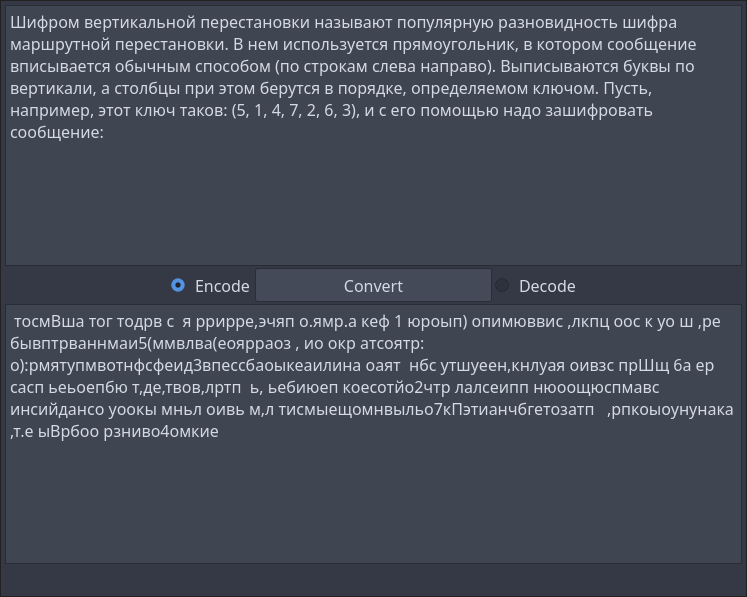
\includegraphics[width=0.7\linewidth]{figures/encode-test-3}}
    \caption{Шифрование}
\label{ris:encode-test-3}
\end{figure}

\vspace{\baselineskip}
\begin{figure}[H]
\center{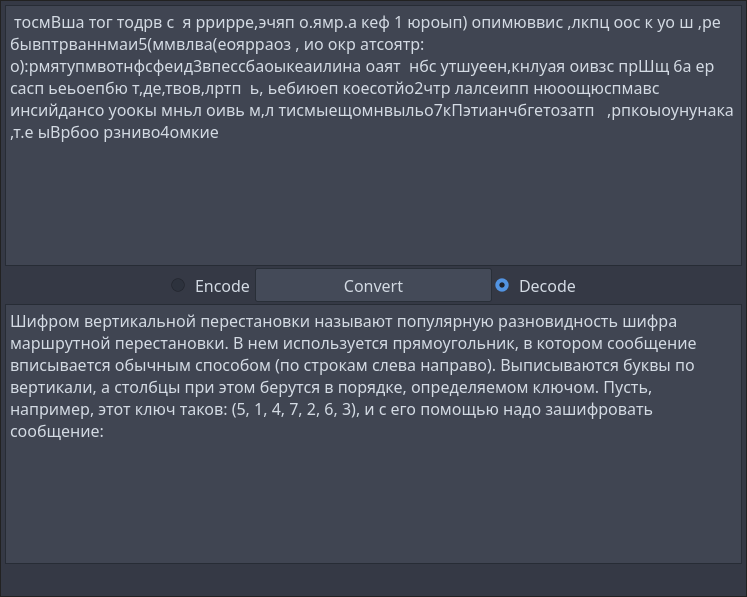
\includegraphics[width=0.7\linewidth]{figures/decode-test-3}}
    \caption{Расшифрование}
\label{ris:decode-test-3}
\end{figure}
